\section{main.cpp File Reference}
\label{main_8cpp}\index{main.cpp@{main.cpp}}
{\tt \#include $<$QApplication$>$}\par
{\tt \#include $<$QSslSocket$>$}\par
{\tt \#include \char`\"{}maindialog.h\char`\"{}}\par


Include dependency graph for main.cpp:\nopagebreak
\begin{figure}[H]
\begin{center}
\leavevmode
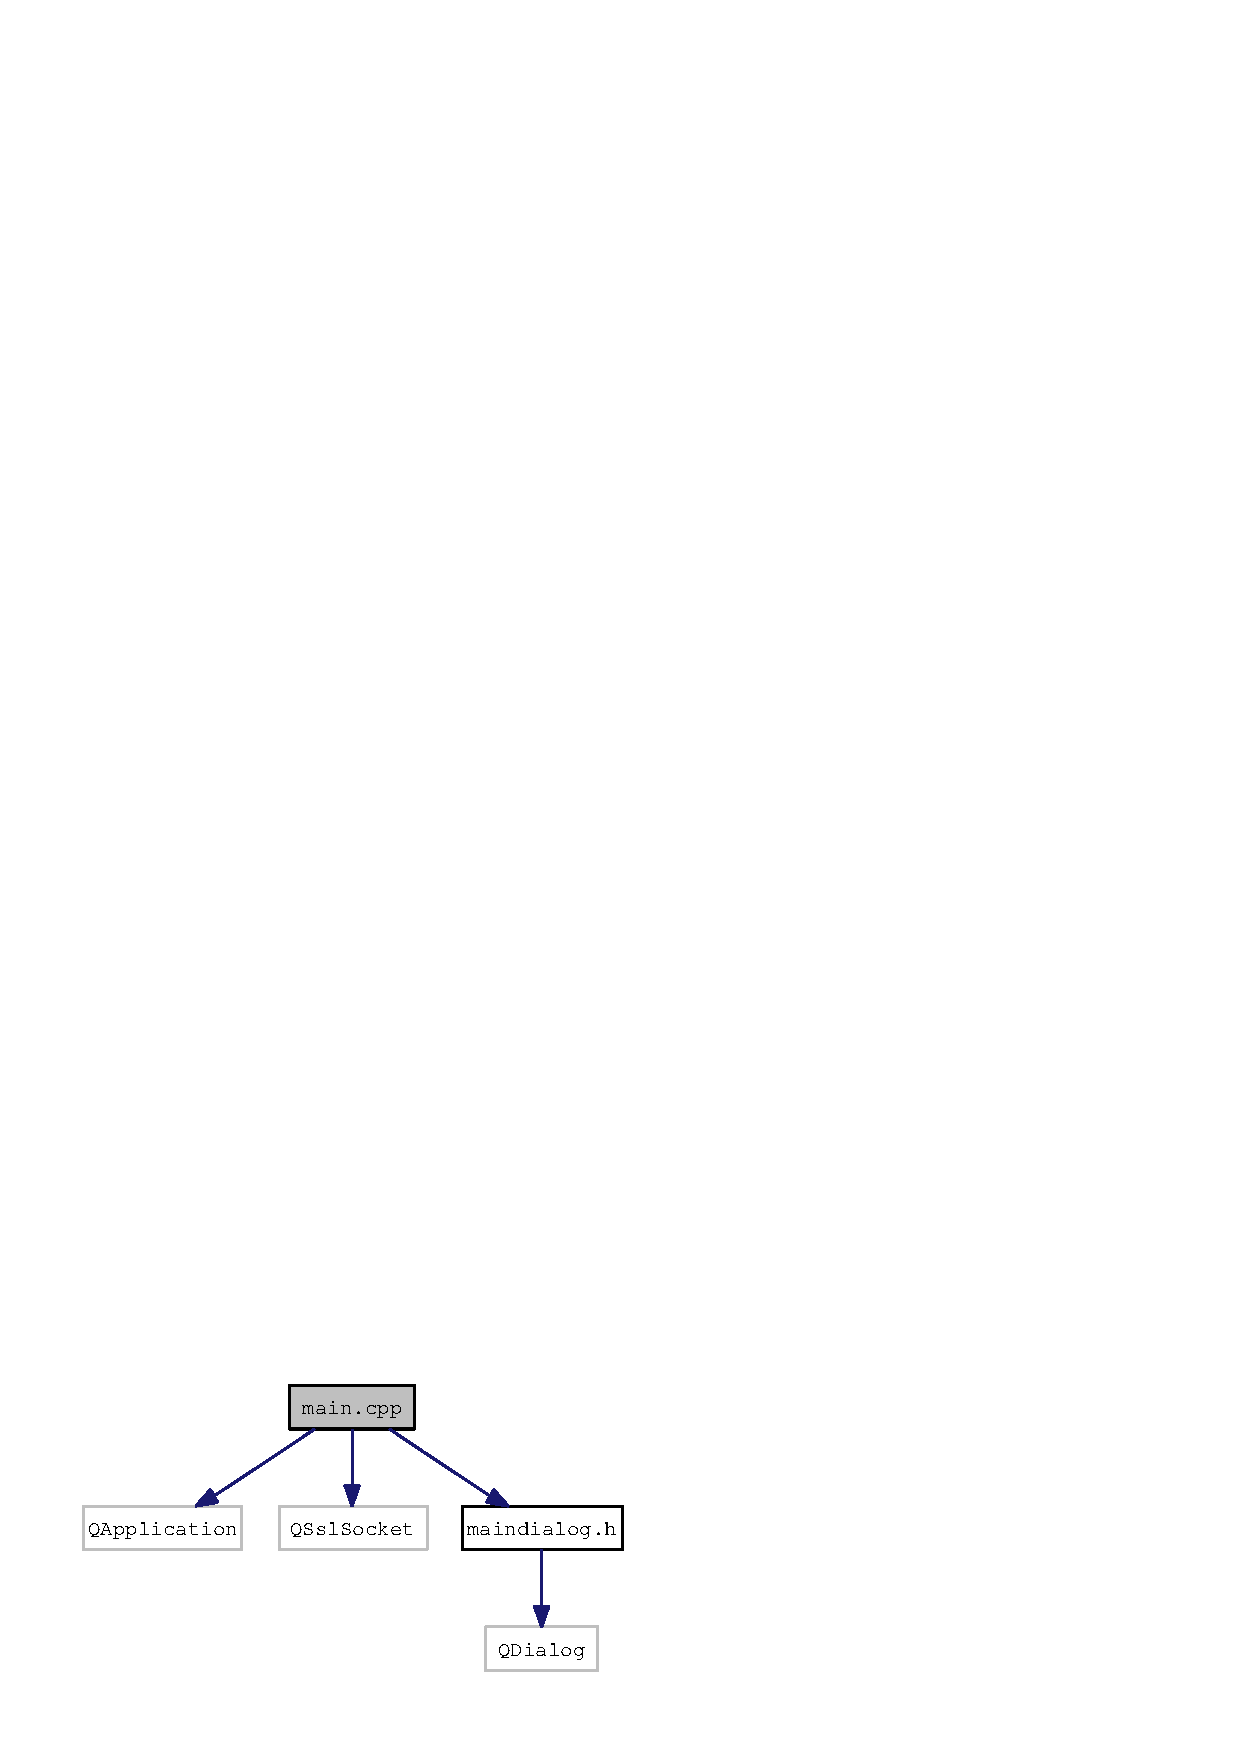
\includegraphics[width=151pt]{main_8cpp__incl}
\end{center}
\end{figure}
\subsection*{Functions}
\begin{CompactItemize}
\item 
int {\bf main} (int argc, char $\ast$$\ast$argv)
\end{CompactItemize}


\subsection{Function Documentation}
\index{main.cpp@{main.cpp}!main@{main}}
\index{main@{main}!main.cpp@{main.cpp}}
\subsubsection{\setlength{\rightskip}{0pt plus 5cm}int main (int {\em argc}, char $\ast$$\ast$ {\em argv})}\label{main_8cpp_3c04138a5bfe5d72780bb7e82a18e627}




Definition at line 5 of file main.cpp.

\begin{Code}\begin{verbatim}6 {
7     if (QSslSocket::supportsSsl()) {
8         QApplication app(argc, argv);
9         MainDialog diag;
10         diag.show();
11         return app.exec();
12     } else {
13         qDebug("No SSL support :(");
14         return 1;
15     }
16 }
\end{verbatim}
\end{Code}


